\section{Composición de funciones}

\begin{figure}[H] 
    \centering    
    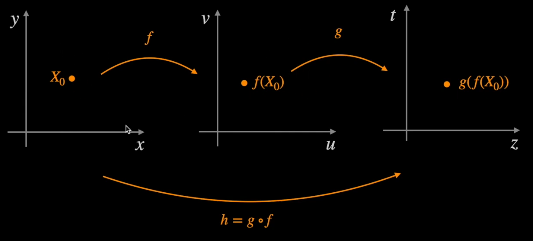
\includegraphics[width=0.6\textwidth]{img/ej-comp-func.png}
    \label{fig:ej-comp-func}
\end{figure}

Para cada $X$, $h(X)$ se define por $h(X) = g \circ f (X) = g(f(X))$

\subsection{Jacobiano}
Sea $\vec{F}:D \subset \mathbb{R}^n \to \mathbb{R}^m$, es diferenciable en $A \in D^\circ$:
$$
\vec{F}(x_1, \ldots, x_n) = (f_1(x_1, \ldots, x_n), \ldots, f_m(x_1, \ldots, x_n))
$$
Se llama matriz Jacobiana de $\vec{F}$ en $A$, y se denota por $D\vec{F}(\vec{A})$, a la matriz:
$$
D\vec{F}(\vec{A}) =
\begin{bmatrix}
\frac{\partial f_1}{\partial x_1} (A) & \cdots & \frac{\partial f_1}{\partial x_n} (A) \\
\vdots & \ddots & \vdots \\
\frac{\partial f_m}{\partial x_1} (A) & \cdots & \frac{\partial f_m}{\partial x_n} (A)
\end{bmatrix}
$$

\begin{figure}[H] 
    \centering    
    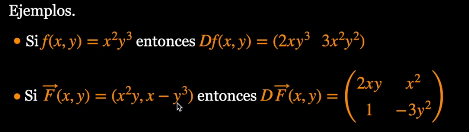
\includegraphics[width=0.5\textwidth]{img/ej-comp-func2.png}
    \label{fig:ej-comp-func2}
\end{figure}

\subsection{Regla de la cadena}
Sea $f:D \subset \mathbb{R}^n \to \mathbb{R}^m$ y 
$g:E \subset \mathbb{R}^m \to \mathbb{R}^p$, y supongamos que $f(D) \subset E$.
Si $f$ es diferenciable en $X_0$ y si $g$ es diferenciable en $f(X_0)$, entonces la función 
compuesta es diferenciable en $X_0$ y se cumple:
$$Dh(X_0) = Dg(f(X_0)) \cdot Df(X_0)$$

\begin{figure}[H] 
    \centering    
    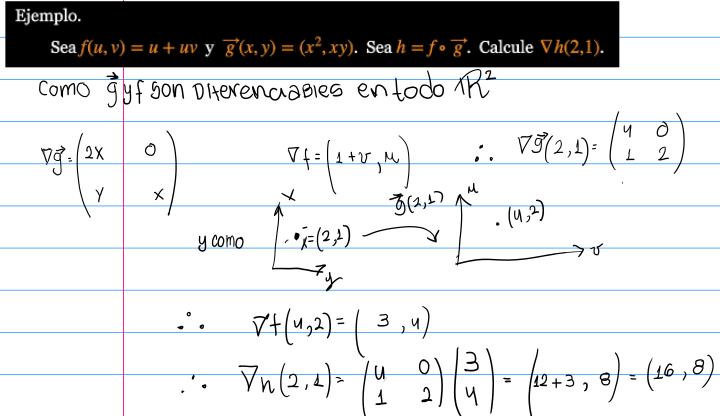
\includegraphics[width=0.7\textwidth]{img/ej-comp-func3.1.png}
    \label{fig:ej-comp-func3.1}
    \caption{Solución I: usando jacobiana.}
\end{figure}
\begin{figure}[H] 
    \centering    
    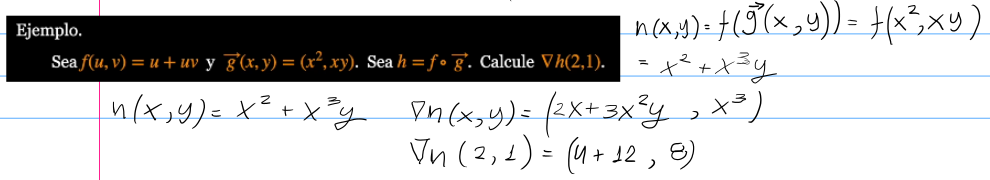
\includegraphics[width=0.7\textwidth]{img/ej-comp-func3.2.png}
    \label{fig:ej-comp-func3.2}
    \caption{Solución II: usando composición.}
\end{figure}

\subsection{Aplicación de la regla de la cadena}
Si $f:D \subset \mathbb{R}^2 \to \mathbb{R}$, $(x_0, y_0) \in D°$ y $f \in Dif(x_0, y_0)$
entonces el gradiente de $f$ en $(x_0, y_0)$ es perpendicular a la curva de nivel de $f$ 
que contiene a $(x_0, y_0)$.
\begin{figure}[H] 
    \centering    
    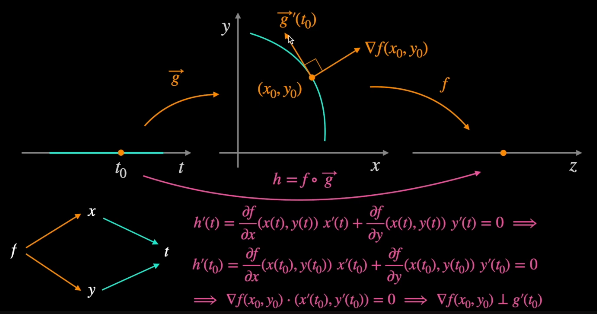
\includegraphics[width=0.7\textwidth]{img/ej-comp-func4.png}
    \label{fig:ej-comp-func4}
\end{figure}